
\chapter{Specifikacija programske potpore}


\section{Funkcionalni zahtjevi}


{Dionici: \begin{packed_enum}
		\item {Voditelj parkirališta (naručitelj)}
		\item {Klijenti}
		\item {Administrator}
		\item {Razvojni tim}
	\end{packed_enum}       
	
	\paragraph*{}{Aktori i njihovi funkcionalni zahtjevi su sljedeći:
	}\begin{packed_enum}
		\item {Voditelj parkirališta može:}
		\begin{packed_item}
			\item {unijeti informacije o svom parkiralištu (naziv, opis, fotografija, cjenik)}
			\item {ucrtati u kartu svako dostupno parkirališno mjesto}
			\item {označiti da je mjesto moguće rezervirati}
			\item {vidjeti informacije o zauzetosti dostupnih parkiralisnih mjesta u realnom vremenu}
			\item {dodati ili obrisati parkirališno mjesto}
		\end{packed_item}
		\item {Neregistrirani korisnik može:}
		\begin{packed_item}
			\item {pregledati na karti dostupna parkirališta i parkirališna mjesta (bez informacije o zauzetosti u stvarnom vremenu)}
			\item {odabrati parkiralište i dobiti prikaz općih informacija (naziv, opis, fotografija, cjenik)}
			\item {poslati zahtjev za registraciju u sustav sa željenom ulogom za koju se prijavljuje (voditelj parkinga ili klijent)}
		\end{packed_item}
		\item {Klijent može:}
		\begin{packed_item}
			\item {vidjeti informacije o zauzetosti dostupnih parkirališnih mjesta u realnom vremenu}
			\item {nadopuniti svoj novčanik}
			\item {odabrati lokaciju svog odredišta, tip vozila i procjenu trajanja parkinga}
			\item {rezervirati parkirališna mjesta označavanjem mjesta na karti}
			\item {rezervirati parkirališna mjesta odabirom označavanjem željenog termina}
		\end{packed_item}
		\item {Administrator može:}
		\begin{packed_item}
			\item {vidjeti popis svih registriranih korisnika i njihovih osobnih podataka}
			\item {vidjeti i promijeniti razinu pristupa aplikaciji korisnicima (klijent, voditelj parkirališta)}
			\item {potvrditi voditelja parkirališta}
			\item {dodati ili obrisati parkiralište}
		\end{packed_item}
	\end{packed_enum}



\subsection{Obrasci uporabe}


\subsubsection{Opis obrazaca uporabe}

\noindent \underbar{\textbf{UC1 - Pregled dostupnih parkirališnih mjesta}}
\begin{packed_item}
	
	\item \textbf{Glavni sudionik: }Klijent
	\item  \textbf{Cilj:} Pregledati dostupna parkirališta i njihovu zauzetost
	\item  \textbf{Sudionici:} Baza podataka
	\item  \textbf{Preduvjet:} Prijava u sustav
	\item  \textbf{Opis osnovnog tijeka:}
	
	\item[] \begin{packed_enum}
		
		\item Klijent ulazi u aplikaciju i pregledava kartu sa svim dostupnim parkiralištima
		\item Klijent bira parkiralište koje ga zanima.
		\item Aplikacija prikazuje informacije o parkiralištu i zauzetosti parkirališnih mjesta na tom parkiralištu.
		
	\end{packed_enum}
	
	\item  \textbf{Opis mogućih odstupanja:}
	
	\item[] \begin{packed_item}
		
		\item[2.a] Klijent odabere parkiralište koje trenutno nema dostupnih slobodnih mjesta.
		\item[] \begin{packed_enum}
			
			\item Aplikacija obavještava klijenta da nema slobodnih mjesta na odabranom parkiralištu.
			
		\end{packed_enum}
		\item[2.b] Klijent pokuša pregledati parkiralište koje ne postoji u sustavu.
		\item[] \begin{packed_enum}
			
			\item Aplikacija obavještava klijenta o nepostojećem parkiralištu.
			
		\end{packed_enum}
		
	\end{packed_item}
	
\end{packed_item}

\noindent \underbar{\textbf{UC2 - Rezervacija parkirališta}}
\begin{packed_item}
	
	\item \textbf{Glavni sudionik: }Klijent
	\item  \textbf{Cilj:} Rezervirati parkiralište za svoje vozilo
	\item  \textbf{Sudionici:} Baza podataka
	\item  \textbf{Preduvjet:} Prijava u sustav
	\item  \textbf{Opis osnovnog tijeka:}
	
	\item[] \begin{packed_enum}
		
		\item Klijent odabire parkiralište na karti i željeni datum i vrijeme rezervacije
		\item Aplikacija prikazuje dostupna slobodna parkirališna mjesta na odabranoj lokaciji za navedeni datum i vrijeme
		\item Klijent odabire slobodno parkirališno mjesto i potvrđuje rezervaciju
		\item Aplikacija omogućuje plaćanje rezervacije
		\item Nakon uspješne rezervacije, klijent prima potvrdu rezervacije putem e-maila
		
	\end{packed_enum}
	
	\item  \textbf{Opis mogućih odstupanja:}
	
	\item[] \begin{packed_item}
		
		\item[2.a] Klijent odabire parkirališne na kojem nema slobodnih mjesta.
		\item[] \begin{packed_enum}
			
			\item Aplikacija obavještava klijenta da na parkiralištu nema slobodnih mjesta.
			
		\end{packed_enum}
		
		\item[3.a] Klijent odabire slobodno parkirališno mjesto koje u međuvremenu postane zauzeto.
		\item[] \begin{packed_enum}
			
			\item Aplikacija obavještava klijenta da se parkiralište promijenilo i predlaže novo slobodno mjesto.
			
		\end{packed_enum}
		
	\end{packed_item}

\end{packed_item}

\noindent \underbar{\textbf{UC3 - Dodavanje informacija o parkiralištu (za voditelje parkinga)}}
\begin{packed_item}
	
	\item \textbf{Glavni sudionik: }Voditelj parkinga
	\item  \textbf{Cilj:} Dodati informacije o svom parkiralištu
	\item  \textbf{Sudionici:} Baza podataka
	\item  \textbf{Preduvjet:} Prijava u sustav kao voditelj parkinga
	\item  \textbf{Opis osnovnog tijeka:}
	
	\item[] \begin{packed_enum}
		
		\item Voditelj parkinga unosi informacije o svom parkiralištu, uključujući naziv, opis, fotografiju, cjenik i sl
		\item Voditelj parkinga može ucrtati svako dostupno parkirališno mjesto za svoje parkiralište
		\item Voditelj parkinga definira je li moguće rezervirati parkirališno mjesto i postavlja senzor koji osvježava informaciju o zauzetosti parkirališnog mjesta
		
	\end{packed_enum}
	
	\item  \textbf{Opis mogućih odstupanja:}
	
	\item[] \begin{packed_item}
		
		\item[1.a] Voditelj parkinga pokuša dodati informacije o parkiralištu koja već postoje u sustavu
		\item[] \begin{packed_enum}
			
			\item Aplikacija obavještava voditelja parkinga o već postojećim informacijama i omogućava izmjenu postojećih podataka
			
		\end{packed_enum}
		\item[3.a] Voditelj parkinga pokušava postaviti senzore na nepostojeće parkiralište.
		\item[] \begin{packed_enum}
			
			\item Aplikacija obavještava voditelja parkinga o nepostojećem parkiralištu i sugerira unos postojećeg parkirališta.
			
		\end{packed_enum}
		
	\end{packed_item}
	
\end{packed_item}

\noindent \underbar{\textbf{UC4 - Statistika zauzetosti parkirališta}}
\begin{packed_item}
	
	\item \textbf{Glavni sudionik: }Voditelj parkinga
	\item  \textbf{Cilj:} Pregledati statistiku zauzetosti parkirališta i parkirališnih mjesta kroz vrijeme
	\item  \textbf{Sudionici:} Baza podataka
	\item  \textbf{Preduvjet:} Prijava u sustav kao voditelj parkinga
	\item  \textbf{Opis osnovnog tijeka:}
	
	\item[] \begin{packed_enum}
		
		\item Voditelj parkinga bira parkiralište za koje želi pregledati statistiku
		\item Aplikacija prikazuje grafički prikaz statistike zauzetosti parkirališta i parkirališnih mjesta tijekom vremena
		
	\end{packed_enum}
	
\end{packed_item}

\noindent \underbar{\textbf{UC5 - Administracija korisnika}}
\begin{packed_item}
	
	\item \textbf{Glavni sudionik: }Administrator
	\item  \textbf{Cilj:} Upravljanje korisnicima i njihovim osobnim podacima
	\item  \textbf{Sudionici:} Baza podataka
	\item  \textbf{Preduvjet:} Prijava u sustav kao administrator
	\item  \textbf{Opis osnovnog tijeka:}
	
	\item[] \begin{packed_enum}
		
		\item Administrator pregledava popis svih registriranih korisnika
		\item Administrator može mijenjati osobne podatke korisnika
		
	\end{packed_enum}
	
	\item  \textbf{Opis mogućih odstupanja:}
	
	\item[] \begin{packed_item}
		
		\item[2.a] Administrator pokušava izmijeniti podatke korisnika na nedozvoljen način.
		\item[] \begin{packed_enum}
			
			\item Sustav obavještava administratora o neispravnoj izmjeni podataka i onemogućava ju.
			
		\end{packed_enum}
		
	\end{packed_item}
	
\end{packed_item}
\newpage
\noindent \underbar{\textbf{UC6 - Prikaz parkirališta za bicikle}}
\begin{packed_item}
	
	\item \textbf{Glavni sudionik: }Klijent
	\item  \textbf{Cilj:}Pregledati dostupna parkirališta za bicikle
	\item  \textbf{Sudionici:} Baza podataka
	\item  \textbf{Preduvjet:} Prijava u sustav
	\item  \textbf{Opis osnovnog tijeka:}
	
	\item[] \begin{packed_enum}
		
		\item Klijent pregledava dostupna parkirališta za bicikle na karti
		\item Aplikacija prikazuje informacije o parkiralištima za bicikle i ukupnom broju slobodnih mjesta
		
	\end{packed_enum}
	
	\item  \textbf{Opis mogućih odstupanja:}
	
	\item[] \begin{packed_item}
		
		\item[2.a] Klijent pregledava parkiralište za bicikle koje trenutno nema slobodnih mjesta
		\item[] \begin{packed_enum}
			
			\item Aplikacija obavještava klijenta da nema slobodnih mjesta na odabranom parkiralištu za bicikle.
			
		\end{packed_enum}
		
	\end{packed_item}
	
\end{packed_item}

\noindent \underbar{\textbf{UC7 - Uplata sredstava u novčanik}}
\begin{packed_item}
	
	\item \textbf{Glavni sudionik: }Klijent
	\item  \textbf{Cilj:}Nadopuniti novčanik sredstvima za plaćanje parkinga
	\item  \textbf{Sudionici:} Bankovni sustav
	\item  \textbf{Preduvjet:} Prijava u sustav
	\item  \textbf{Opis osnovnog tijeka:}
	
	\item[] \begin{packed_enum}
		
		\item Klijent odabire opciju za uplatu sredstava
		\item Klijent unosi iznos koji želi uplatiti
		\item Aplikacija preusmjerava korisnika na sigurnu stranicu za plaćanje gdje unosi bankovne podatke
		\item Nakon uspješne uplate, sredstva se dodaju u novčanik korisnika
		
	\end{packed_enum}
	
	\item  \textbf{Opis mogućih odstupanja:}
	\item[] \begin{packed_item}
		
		\item[3.a] Klijent pokušava izvršiti uplatu, ali bankovni sustav ne uspijeva obraditi transakciju
		\item[] \begin{packed_enum}
			
			\item Klijent prima obavijest o neuspjeloj uplati i dobiva priliku ponovno pokušati uplatu.
			
		\end{packed_enum}
		
	\end{packed_item}
	
\end{packed_item}
\newpage
\noindent \underbar{\textbf{UC8 - Registracija}}
\begin{packed_item}
	
	\item \textbf{Glavni sudionik: } Neregistrirani korisnik
	\item  \textbf{Cilj:} Stvoriti korisnički račun za pristup aplikaciji
	\item  \textbf{Sudionici:} Baza podataka
	\item  \textbf{Preduvjet:} -
	\item  \textbf{Opis osnovnog tijeka:}
	
	\item[] \begin{packed_enum}
		
		\item Korisnik odabire opciju za registraciju
		\item Korisnik unosi potrebne korisnčke podatke
		\item Korisnik prima obavijest o uspješnoj registraciji
		
	\end{packed_enum}
		\item  \textbf{Opis mogućih odstupanja:}
	\item[] \begin{packed_item}
		
		\item[2.a] Odabir već zauzetog korisničkog imena i/ili e-maila, unos korisničkog podatka u nedozvoljenom formatu ili pružanje neispravnoga e-maila
		\item[] \begin{packed_enum}
			
			\item {Sustav obavještava korisnika o neuspjelom upisu i vraća ga na stranicu za registraciju} 
			
			\item {Korisnik mijenja potrebne podatke te završava unos ili odustaje od registracije}
		\end{packed_enum}
		
	\end{packed_item}
	
\end{packed_item}

\newpage

\subsection{Dijagrami obrazaca uporabe}



% TODO: \usepackage{graphicx} required
\begin{figure}[!htb]
	\centering
	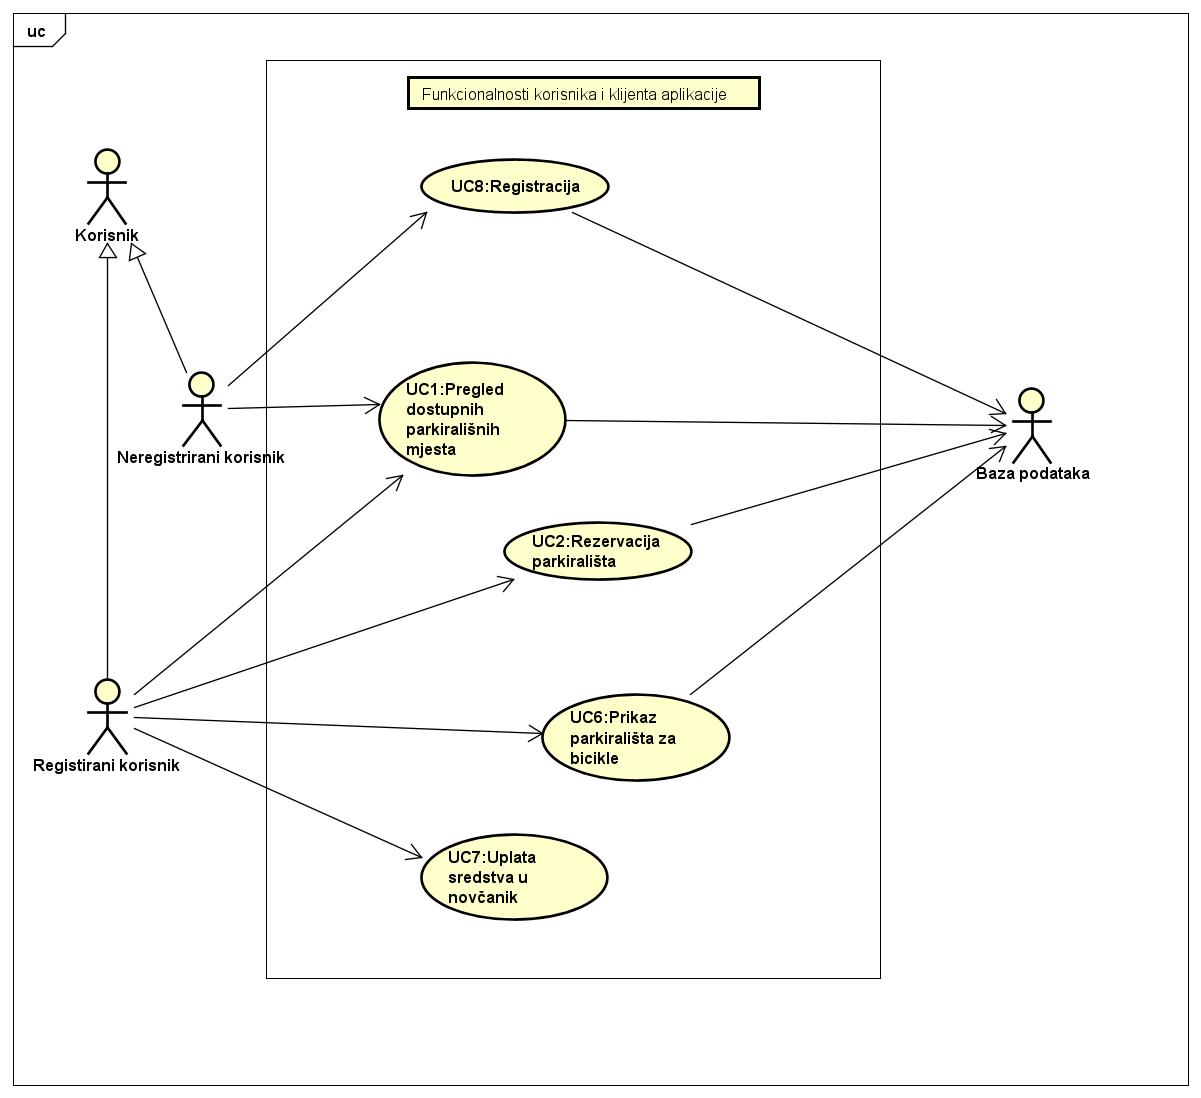
\includegraphics[width=1\linewidth]{dijagrami/dijagramKlijent.jpg}
	\caption{ Dijagram obrasca uporabe, funkcionalnost korisnika i klijenta}
	\label{fig:dijagramklijent}
	
\end{figure}

% TODO: \usepackage{graphicx} required
\begin{figure}[!htb]
	\centering
	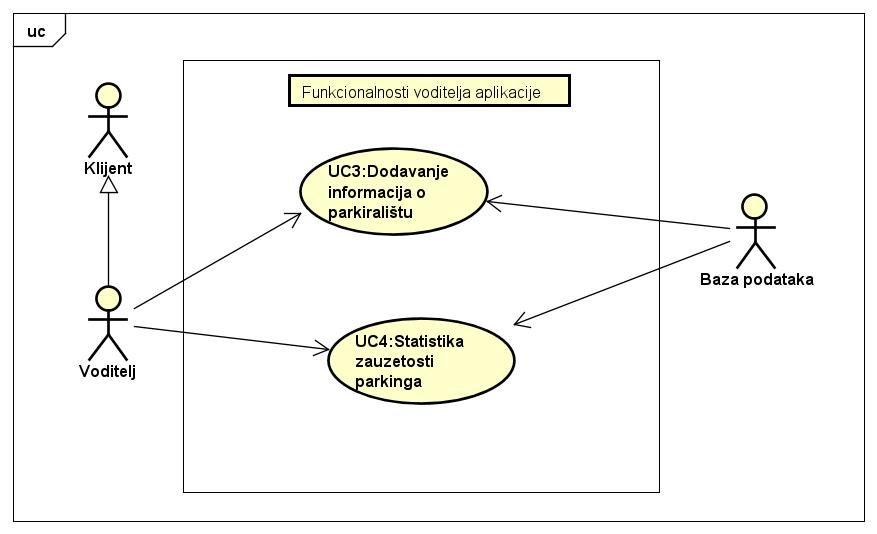
\includegraphics[width=1\linewidth]{dijagrami/dijagramVoditelj}
	\caption{Dijagram obrasca uporabe, funkcionalnost vlasnika}
	\label{fig:dijagramvoditelj}
\end{figure}

% TODO: \usepackage{graphicx} required
\begin{figure}[!htb]
	\centering
	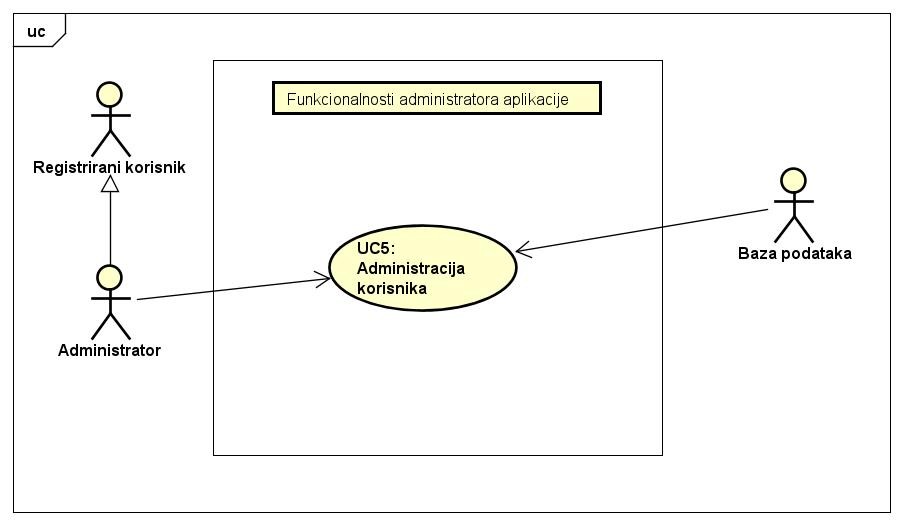
\includegraphics[width=1\linewidth]{dijagrami/dijagramAdmin}
	\caption{Dijagram obrasca uporabe, funkcionalnost administratora}
	\label{fig:dijagramadmin}
\end{figure}




\newpage
	
\subsection{Sekvencijski dijagrami}

\subsubsection{Obrazac uporabe UC1 - Pregled dostupnih parkirališta}

{Klijent šalje zahtjev za kartografskim prikazom s dostupnim parkiralištima kako bi odabrao parkiralište.Aplikacija dohvaća trenutne podatke o svim parkiralištima iz baze podataka i prikazuje ih korisniku.Nakon što klijent odabere parkiralište na karti, aplikacija šalje upit bazi podataka kako bi dohvatila osnovne informacije o odabranom parkiralištu.Baza podataka odgovara na upit i šalje informacije o parkiralištu i zauzetosti parkirališnih mjesta, što aplikacija prikazuje korisniku.}

% TODO: \usepackage{graphicx} required
\begin{figure}[!htb]
	\centering
	\includegraphics[width=1\linewidth]{"dijagrami/UC1 - Pregled dostupnih parkirališta"}
	\caption{Sekvencijski dijagram za UC1}
	\label{fig:uc1---pregled-dostupnih-parkiralista}
\end{figure}


\subsubsection{Obrazac uporabe UC2 -Rezervacija parkirališta}

{Klijent šalje zahtjev za rezervaciju parkirališta odabirom parkirališta na karti i specificiranjem datuma i vremena rezervacije.Aplikacija šalje upit bazi podataka kako bi provjerila dostupnost slobodnih parkirališnih mjesta na odabranoj lokaciji za navedeni datum i vrijeme.Baza podataka provjerava dostupna mjesta i šalje informacije o slobodnim parkirališnim mjestima aplikaciji.Ako nema slobodnih mjesta na odabranom parkiralištu aplikacija obavještava klijenta o tome uz poruku.Aplikacija prikazuje klijentu dostupna slobodna mjesta i omogućuje odabir.Klijent bira slobodno parkirališno mjesto i potvrđuje rezervaciju.Aplikacija šalje upit bazi podataka za rezervaciju parkirališta.Baza podataka rezervira parkiralište i šalje potvrdu rezervacije aplikaciji.Aplikacija omogućuje klijentu plaćanje rezervacije.Aplikacija šalje potvrdu plaćanja bazi podataka.Baza podataka ažurira status rezervacije i potvrđuje plaćanje.Aplikacija šalje potvrdu rezervacije klijentu.Klijent prima potvrdu rezervacije.}


% TODO: \usepackage{graphicx} required
\begin{figure}[!htb]
	\centering
	\includegraphics[width=1\linewidth]{"dijagrami/UC2 - Rezervacija Parkirališta"}
	\caption{Sekvencijski dijagram za UC2}
	\label{fig:uc2---rezervacija-parkiralista}
\end{figure}

\newpage

\section{Ostali zahtjevi}
	\begin{packed_item}
		\item {Sustav treba omogućiti rad više korisnika u stvarnom vremenu}
		\item {Korisničko sučelje i sustav moraju podržavati hrvatsku abecedu (dijakritičke znakove) pri unosu i prikazu tekstualnog sadrzaja}
		\item {Izvršavanje dijela programa u kojem se pristupa bazi podataka ne smije trajati duže od nekoliko sekundi}
		\item {Sustav treba biti implementiran kao web aplikacija koristeći objektno-orijentirane jezike}
		\item {Sustav treba biti jednostavan za korištenje, korisnici se moraju znati koristiti sučeljem bez opširnih uputa }
		\item {Sustav kao valutu koristi EURO}
		\item {Veza s bazom podataka mora biti kvalitetno zaštićena, brza i otporna na vanjske greške}
		\item {Pristup sustavu mora biti omogućen iz javne mreže pomoću HTTPS}
	\end{packed_item}



\eject

	
